\documentclass[a4paper, 10pt]{article}

\usepackage[utf8x]{inputenc}
\usepackage[english, russian, ukrainian]{babel}
\usepackage{cmap}
\usepackage{mathtext}
\usepackage[T2A]{fontenc}

\usepackage{graphicx}
\usepackage{float}
\usepackage{listings}

\usepackage{geometry}
\geometry{top = 2cm}
\geometry{bottom = 2cm}
\geometry{left = 3cm}
\geometry{right = 1.5cm}

\begin{document}
\begin{titlepage}
\begin{center}
\large{
Міністерство освіти і науки, молоді та спорту України\\
Національний технічний університет України\\
``Київський політехнічний інститут''\\
Факультет прикладної математики\\
Кафедра спеціалізованих комп’ютерних систем\\
}

\vfill

\large{\bf{
Лабораторна робота №3\\
Дисципліна:\\
``Архітектура комп'ютерів''\\
Тема:\\
``Вивчення роботи обчислювальної системи керованою потоком даних''\\
}}

\vfill

\begin{table}[h]
\centering
\begin{tabular}{lp{4cm}l}
Виконав:&&Перевірив:\\
Студент групи КВ--92&&Жабін В. І.\\
Гуль О. В.&&\\
Залікова книжка № КВ--9203&&\\
\end{tabular}
\end{table}

\vfill

Київ \the\year
\end{center}
\end{titlepage}
\newpage

\section{Мета}
Вивчити роботу ОС, побудовану на основі буферної пам'яті даних і на основі асоціативної пам'яті. Визначити характеристики вказаних систем.

\section{Завдання}
\begin{enumerate}
    \item Вивчити ОС з буферною пам'яттю даних і з асоціативною пам'яттю. При вивченні звернути увагу на формат даних і специфіку програмування. Так само при вивченні ОС з буферною пам'яттю даних звернути увагу на алгоритми опиту буферної пам'яті.
    \item Визначити 7 молодших розрядів двійкового представлення номера залікової книжки.
    \item Згідно з цими цифрам визначити свій варіант лабораторної роботи.
    \item Визначити ЯПФ кожної функції.
    \item Виконати адресацію всіх операцій, враховуючи, що всі 3 функції виконуватимуться спільно.
    \item Написати програму сумісного виконання всіх функцій (Підказка: для ефективнішої роботи порядок введення повинен забезпечувати ``горизонтальне'' введення, тобто команди повинні потрапляти в систему по ярусах, а не по вітках. І краще, якщо реалізовувати введення по ярусах всіх трьох (N) функцій).
\end{enumerate}

\noindent
Варіант: $9203=10001111110011_2.$\\
$a_{6},\cdots,a_{0}=1110011.$\\
Набір функцій: $f2, f3, f4.$\\
Кількість пристроїв введення: $5.$\\
Примітка: розміщення слів для введення виконати самостійно, враховуючи особливості алгоритму.\\
Виведення на пристрій: $1, 2, 4.$\\
Примітка: Для всіх варіантів кількість пристроїв виводу~-- 4.\\

\noindent
$f2 = \sqrt{5a + b + c^2} + 2ac$\\
$f3 = a - b - ac + 12\sqrt{a^2 + b^2}$\\
$f4 = ab(a^2 + b^2 + c^2 + d^2)$\\

Дані для всіх функцій задати самостійно.

\section{Порядок виконання роботи}
\begin{enumerate}
    \item Набрати в редакторові програму. Запустити її на виконання і перевірити правильність виконання функцій. У разі потреби можна знайти помилки, використовуючи відладчик.
    \item {
	Дослідження системи.
	\begin{enumerate}
	    \item Встановити в ``Набір операцій'' великі значення кількості кроків виконання операцій (приблизно 30) і в ``параметрах системи'' мінімально можливі значення кількості обчислювальних пристроїв (1) і розмірів БПД і БПК (2). Запустити програму на автоматичне виконання при алгоритмі опиту ``Послідовний по порядку введення'', а потім ``с вільним осередком БПД''. Зробити висновки.

	    \item Міняючи розмір буферів і кількості процесорів добитися максимальної продуктивності системи на програмі. Визначити кількість обчислювальних блоків, при якій подальше нарощування не дає виграшу в продуктивності.

	    \item Зменшуючи кількість процесорів визначити динаміку зменшення продуктивності, визначаючи на кожному кроці $К_{у} = Т_{1} / Т_{i}$, де $Т$~-- кількість тактів виконання програми.

	    \item Повторити попередній пункт для системи з асоціативною пам'яттю, розібратися в специфіці системи і порівняти характеристики з  системою з буферною пам'яттю даних. Зробити висновки.
	\end{enumerate}
}

	\item Зробити висновки по роботі.
\end{enumerate}

\section{Виконання завдання}
\begin{figure}[H]
\begin{center}
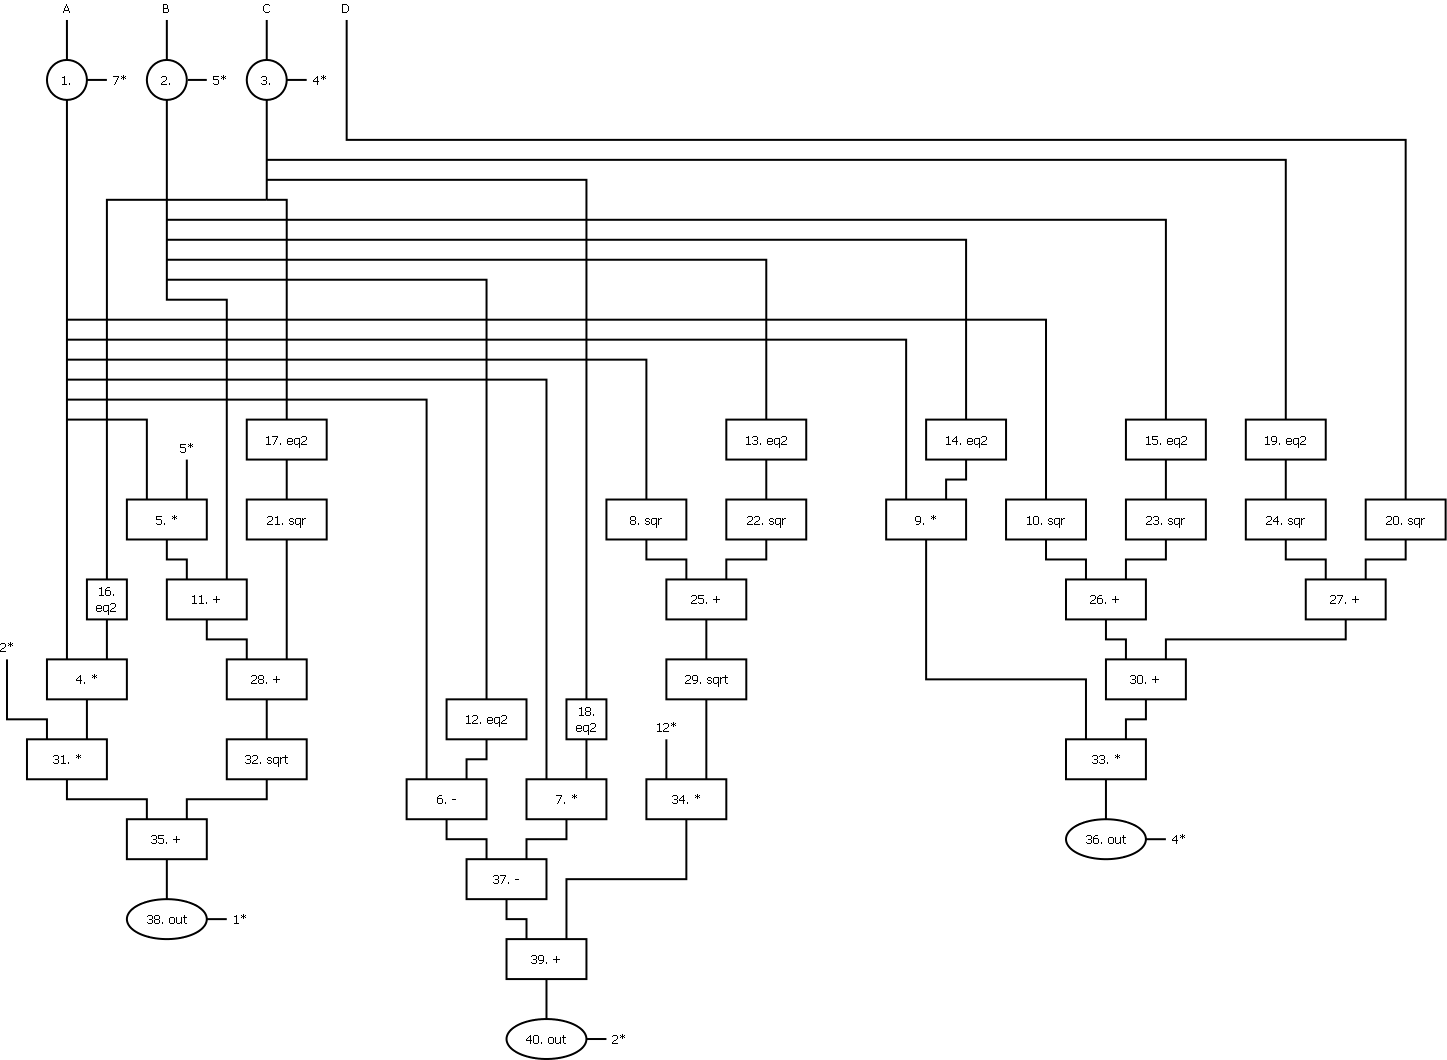
\includegraphics[scale=0.3, angle=90]{lab3_alg.png}
\caption{Граф програми обчислення.}
\end{center}
\end{figure}

\begin{figure}[H]
\begin{center}
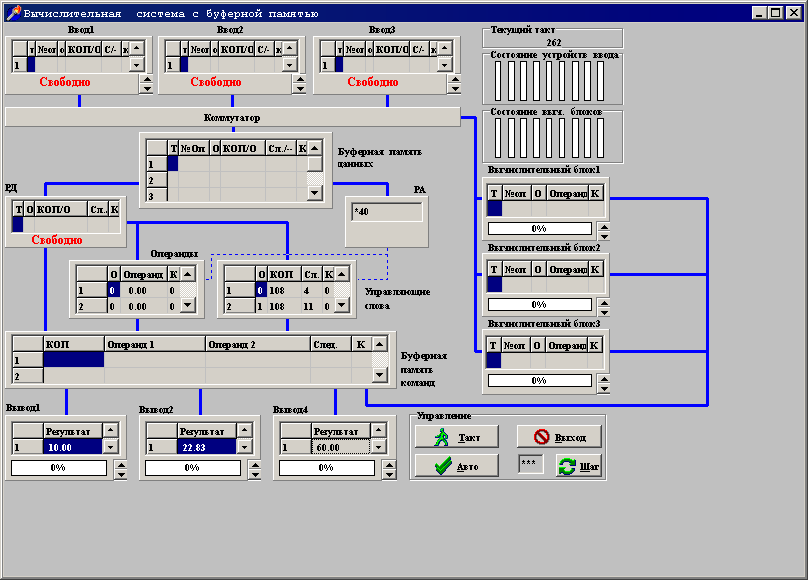
\includegraphics[scale=0.75]{lab3.png}
\caption{Результат виконання.}
\end{center}
\end{figure}

lab3.asm
\begin{lstlisting}[numbers=left]
program lab3
constant
a = 1
b = 2
c = 3
d = 4
begin
 1: xn    a,  7, !0 to  4
 2: xn    b,  5, !1 to 11
 3: xn    c,  4, !1 to 16
 4: mul   _,  _, !1 to 31
 5: mul   _, 5*, !0 to 11
 6: sub   _,  _, !0 to 37
 7: mul   _,  _, !1 to 37
 8: sqr   _, 0*, !0 to 25
 9: mul   _,  _, !0 to 33
10: sqr   _, 0*, !0 to 26
11: add   _,  _, !0 to 28
12: eq2  0*,  _, !1 to  6
13: eq2  0*,  _, !0 to 22
14: eq2  0*,  _, !1 to  9
15: eq2  0*,  _, !0 to 23
16: eq2  0*,  _, !1 to  4
17: eq2  0*,  _, !0 to 21
18: eq2  0*,  _, !1 to  7
19: eq2  0*,  _, !0 to 24
20: sqr   d, 0*, !1 to 27
21: sqr   _, 0*, !1 to 28
22: sqr   _, 0*, !1 to 25
23: sqr   _, 0*, !1 to 26
24: sqr   _, 0*, !0 to 27
25: add   _,  _, !0 to 29
26: add   _,  _, !0 to 30
27: add   _,  _, !1 to 30
28: add   _,  _, !0 to 32
29: sqrt  _, 0*, !1 to 34
30: add   _,  _, !1 to 33
31: mul  2*,  _, !0 to 35
32: sqrt  _, 0*, !1 to 35
33: mul   _,  _, !0 to 36
34: mul 12*,  _, !1 to 39
35: add   _,  _, !0 to 38
36: out   _, 4*, !0 to 36
37: sub   _,  _, !0 to 39
38: out   _, 1*, !0 to 38
39: add   _,  _, !0 to 40
40: out   _, 2*, !0 to 40
end
\end{lstlisting}

Результат отриманий для:\\
\begin{itemize}
	\item Кількість пристроїв введення: 5.
	\item Кількість пристроїв виведення: 4.
	\item Кількість процесорів: 16.
	\item Довжина буферної пам'яті даних: 16.
	\item Довжина буферної пам'яті команд: 16.
	\item Розмір пам'яті: 128.
	\item Параметри часу виконання команд~-- стандартні.
	\item Алгоритм опитування: з вільною коміркою БПД.
	\item Система: з буферною пам'яттю.
\end{itemize}

\section{Результати досліджень}
\begin{enumerate}
	\item В даних умовах програма зависає при будь--якому алгоритмі опитування.
	\item Кількість процесорів: 12, розмір БПД і БПК: 2.
	\item {
		\begin{table}[H]
		\centering
		\begin{tabular}{|c|c|c|}
		\hline
		Кількість процесорів & час виконання & K \\
		\hline
		12 & 262 & 1      \\
		11 & 264 & 1.0076 \\
		10 & 264 & 1.0076 \\
	 	 9 & 266 & 1.0153 \\
		 8 & 266 & 1.0153 \\
		 7 & 266 & 1.0153 \\
		 6 & 266 & 1.0153 \\
		 5 & 270 & 1.0305 \\
		 4 & 295 & 1.1260 \\
		 3 & 348 & 1.3282 \\
		 2 & 471 & 1.7977 \\
		 1 & 857 & 3.2710 \\
		\hline
		\end{tabular}
		\caption{Динаміка зменшення продуктивності для системи з буферною пям'яттю.}
		\end{table}
	}

	\item {
		\begin{table}[H]
		\centering
		\begin{tabular}{|c|c|c|}
		\hline
		Кількість процесорів & час виконання & K \\
		\hline
		12 & 262 & 1      \\
		11 & 264 & 1.0076 \\
		10 & 264 & 1.0076 \\
	 	 9 & 267 & 1.0191 \\
		 8 & 267 & 1.0191 \\
		 7 & 267 & 1.0191 \\
		 6 & 267 & 1.0191 \\
		 5 & 269 & 1.0267 \\
		 4 & 314 & 1.1985 \\
		 3 & 363 & 1.3855 \\
		 2 & 473 & 1.8053 \\
		 1 & 859 & 3.2786 \\
		\hline
		\end{tabular}
		\caption{Динаміка зменшення продуктивності для системи з асоціативною пям'яттю.}
		\end{table}
	}
\end{enumerate}

\section{Висновки}
При виборі параметрів системи потрібно відщтовхуватись від складності задачі, тому що можна допустити зависання програми.\\
З додаванням кожного нового обчислювального блоку пришвидшення виконання зменшується.
\end{document}
